\subsection{Imágenes}

Las siguientes implementaciones operan con imágenes del tipo bmp y canales $alfa$, $red$, $green$ y $blue$ ($argb$) de 8 bits cada uno (de ahí la variante bmp 32 bits).\\

En memoria los datos de cada pixel estarán ordenados a la inversa, es decir, $bgra$, por lo cual al trabajarlos en registros de procesador, los mismos serán invertidos debido a que es el formato standard utilizado por la arquitectura intel para almacenar datos en memoria.
El puntero de fuente obtenido en todas las implementaciones representa a la imagen a la cual se le quiere aplicar el filtro. La misma tiene una particularidad para la lectura y es que la primera fila leida es la última de la imagen.\\

Llamaremos $O$ a la imagen de salida generada por cada filtro. Por ejemplo, el filtro identidad
estaría caracterizado por la fórmula\\

\begin{center}
$\forall$ $k$ $\in$ ($r, g, b, a$) $O^{k}_{i,j}$ = $I^{k}_{i,j}$
\end{center}

\subsection{Implementaciones}
Introduciremos cada filtro mencionandolos en el siguiente orden:
 
\begin{enumerate}
\item Cropflip
\item Sepia
\item Low dynamic range 
\end{enumerate}

Para cada uno expondremos su idea principal, es decir, que efecto tiene sobre la imagen a la que se aplica, mostrando un caso de ejemplo. Luego expondremos las implementaciones, focalizando y detallando principalmente la implementación en lenguaje assembler SIMD.

\subsection{Cropflip}
Este filtro es una unión de dos filtros: crop y vertical-flip. Al aplicarlo sobre una imagen, recorta una parte de la misma y la voltea verticalmente. Para ello recibe cuatro argumentos delimitando un rectangulo de la imagen.

\begin{itemize}
\item{$tamx$: Posee la cantidad de columnas, en pixeles, a recortar. Este número es multiplo de 4.}
\item{$tamy$: Contiene la cantidad de filas, en pixeles, a recortar.}
\item{$offseex$: Columna, en pixeles, a partir de la cual se debe comenzar a recortar. Este número también es multiplo de 4.}
\item{$offsety$: Fila, en pixeles, a partir de la cual se debe comenzar a recortar.}
\end{itemize}

El recuadro obtenido se devuelve espejadolo verticalmente. Para ello rearma las filas en orden inverso.\\

\newpage

\begin{figure}[h]
  \centering
  \subfloat[Original]{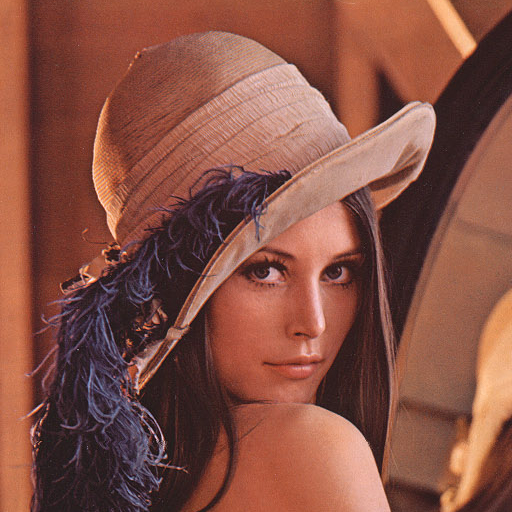
\includegraphics[width=0.4\textwidth]{imagenes/lena32.jpg}\label{fig:f1}}
  \hfill
  \subfloat[Cropflip]{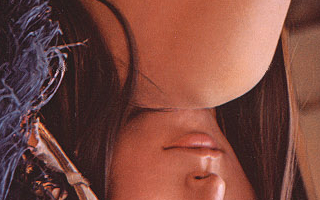
\includegraphics[width=0.4\textwidth]{imagenes/lena32cropflip.jpg}\label{fig:f2}}
  \caption{Corte: 320x200 $offset x: 100$ y $offset y: 0$}
\end{figure}

Si bien es el código más sencillo de implementar, incluso de manera eficiente, requiere algún tipo de explicación.

\subsubsection{Assembler SIMD}

En la implementación de SIMD se aprovecha el uso de paralelismo y la capacidad de almacenar hasta cuatro pixeles en un registro $xmm$.\\ 
Tomando entonces de a 4 pixeles, desde el inicio del rectangulo determinado por los parametros, se rearma la imagen, logrando finalmente, al recorrer todas las filas indicadas, el espejado vertical esperado.

\begin{codesnippet}
\begin{verbatim}
.ciclo:
        movdqu xmm1, [rdi]      ; p0|p1|p2|p3
        movdqu [rsi], xmm1
    
        lea rsi, [rsi + 16]
        lea rdi, [rdi + 16]
        loop .ciclo
\end{verbatim}
\end{codesnippet}

Como puede observarse, mediante un ciclo podemos con la ayuda de un registro xmm transportar desde la fuente hasta el destino, 4 pixeles simultaneamente, que corresponde en total a la fila de la imagen.

\subsubsection{C}

En principio, C compilado sin flags de optimización (es decir compilado con $O0$, modo default) el código final se resuelve puramente con instrucciones de assembler. Por lo tanto cada pixel se opera unitariamente. 

\begin{codesnippet}
\begin{verbatim}
    for (int i = 0; i < tamy; i++) 
    {
        for (int j = 0; j < tamx; j++) 
        {

            bgra_t *p_d = (bgra_t*) &dst_matrix[(tamy-1)-i][j*4];
            bgra_t *p_s = (bgra_t*) &src_matrix[i+offsety][(j+offsetx)*4];

            p_d->b = p_s->b;
            p_d->g = p_s->g;
            p_d->r = p_s->r;
            p_d->a = p_s->a;

        }
    }
\end{verbatim}
\end{codesnippet}

\subsection{Sepia}
Esta operación consiste en cambiar la información de color de cada pixel de la siguiente manera:

\begin{center}
$$O_{i,j}^{R} = 0, 5 . suma_{i,j}$$
$$O_{i,j}^{G} = 0, 3 . suma_{i,j}$$
$$O_{i,j}^{B} = 0, 2 . suma_{i,j}$$
\end{center}

donde 

\begin{center}
$suma_{i,j} = I_{i,j}^{R} + I_{i,j}^{G} + I_{i,j}^{B}$
\end{center}

El efecto logrado es que realza más el canal verde. 

\newpage

\begin{figure}[h]
  \centering
  \subfloat[Original]{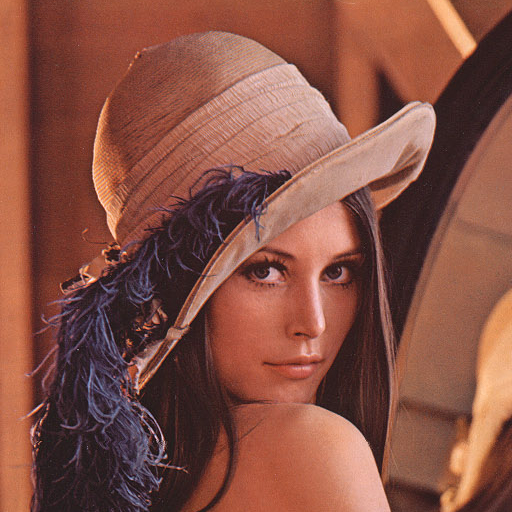
\includegraphics[width=0.4\textwidth]{imagenes/lena32.jpg}\label{fig:f3}}
  \hfill
  \subfloat[Sepia]{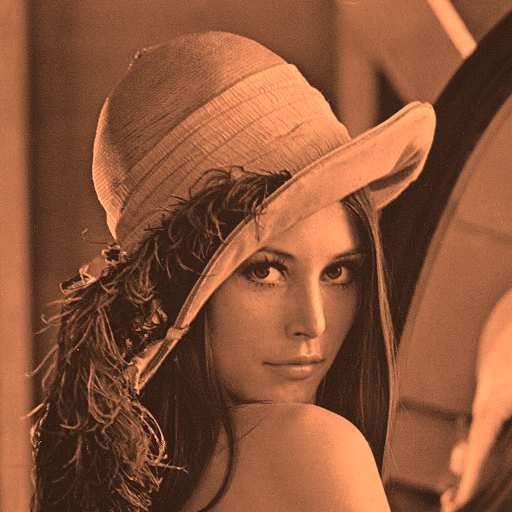
\includegraphics[width=0.4\textwidth]{imagenes/lena32sepia.jpg}\label{fig:f4}}
\end{figure}

Si bien es una operación sencilla, los tiempos de cómputo se ven comprometidos para imágenes muy grandes debido a la cantidad de operaciones en punto flotante: En una imagen de 512x512 pixeles tenemos 512x512x3 = 786432 operaciones de punto flotante. Lo cual puede suponer un desafio si no se dispone de tecnologias como SIMD.

\subsubsection{Assembler SIMD}

Al igual que en el primer filtro, se aprovecha el paralelismo de SIMD para el cálculo en punto flotante.\\

Para operar la imagen se procesa de a 4 pixeles. Luego cada pixel se lleva a un registro $xmm$ extendiendo sus canales a 32 bits. Como no se asume que el alfa sea cero se utiliza una máscara para borrarlo previemente. Luego se realiza la suma de los canales para cada pixel y por último se convierte cada una a punto flotante 32 bits y se realizan los 3 productos para cada suma que corresponden a los nuevos canales $r$, $g$ y $b$ mediante el uso de operaciones de punto flotante.\\

Al final se restaura el canal alfa junto con el nuevo pixel calculado y se devuelve a la imagen destino. 

\begin{codesnippet}
\begin{verbatim}
factores: DD  0.2, 0.3, 0.5, 0.0 
alfamasc: DB  0, 0, 0, 0XFF, 0, 0, 0, 0XFF, 0, 0, 0 , 0XFF, 0, 0, 0, 0XFF
alfainv: DB 0xFF, 0xFF, 0xFF, 0, 0xFF, 0xFF, 0xFF, 0, 0xFF, 0xFF, 0xFF, 0, 0xFF, 0xFF, 0xFF, 0    
section .text

;Notacion:
;px = pixel input 
;sumax = sumatoria de las componentes de px
;px' = pixel output deseado
;El contenido de los registros XMM se muestra del 
;	bit mas significativo al menos significativo

_sepia_asm:
	;rdi *src
	;rsi *dst
	;edx int cols
	;ecx int filas
	;r8d int src_row_size
	;r9d int dst_row_size

	push rbp
	mov rbp, rsp
	
	mov eax, edx
	mul ecx
	mov ecx, eax
	sar ecx, 2; ecx/4 me muevo cuatro pixeles por iteracion

 	movdqu xmm7, [alfainv] ; XMM7 = | 00 | FF | FF | FF |...
	movdqu xmm8, [alfamasc]; XMM8 = | FF | 00 | 00 | 00 |...
	movups xmm0, [factores]
	pxor xmm6, xmm6	

	.ciclo:	
		movdqu xmm1, [rdi]; XMM1 = | p3 | p2 | p1 | p0 |
		movdqu xmm2, xmm1 ; XMM1 = XMM2
		movdqu xmm5, xmm1; respaldo XMM5 = XMM1

		;limpiar alfa
		pand xmm1, xmm7; XMM1 = | 0 | r3 | g3 | b3 |...
		pand xmm2, xmm7; idem
			
			
		punpcklbw xmm1, xmm6; XMM1 = | p1 | p0 | con alfa limpio
		punpckhbw xmm2, xmm6; XMM2 = | p3 | p2 | con alfa limpio
		
		movdqu xmm3, xmm1
		movdqu xmm4, xmm2
		punpcklbw xmm1, xmm6; XMM1 = | 0 | r0 | g0 | b0 |
		punpckhbw xmm3, xmm6; XMM3 = | 0 | r1 | g1 | b1 |
		punpcklbw xmm2, xmm6; XMM2 = | 0 | r2 | g2 | b2 |
		punpckhbw xmm4, xmm6; XMM4 = | 0 | r3 | g3 | b3 |

\end{verbatim}
\end{codesnippet}

\begin{codesnippet}
\begin{verbatim}
		phaddd xmm1, xmm1; XMM1 = | r0 | g0 + b0 | r0 | g0 + b0 |
		phaddd xmm1, xmm1; XMM1 = | suma0 | suma0 | suma0 | suma0 | 
		phaddd xmm2, xmm2; idem con pixeles 1, 2 y 3
		phaddd xmm2, xmm2
		phaddd xmm3, xmm3 
		phaddd xmm3, xmm3
		phaddd xmm4, xmm4
		phaddd xmm4, xmm4

		; un unpack mas, multiplico de a un pixel

		cvtdq2ps xmm1, xmm1;  suma0 asFloat
		cvtdq2ps xmm2, xmm2;  suma2 asFloat
		cvtdq2ps xmm3, xmm3;  suma1 asFloat
		cvtdq2ps xmm4, xmm4;  suma3 asFloat

		; xmmm0 tiene la mascara con los valores 0.2 0.3 0.5 0.0
		mulps xmm1, xmm0; XMM1 = |*|suma0*0.2|suma0*0.3|suma0*0.5|  
		mulps xmm2, xmm0; XMM2 = |*|suma2*0.2|suma2*0.3|suma2*0.5|  
		mulps xmm3, xmm0; XMM3 = |*|suma1*0.2|suma1*0.3|suma1*0.5|   
		mulps xmm4, xmm0; XMM4 = |*|suma3*0.2|suma3*0.3|suma3*0.5|   

		cvttps2dq xmm1, xmm1; |0|suma0*0.2 asInt|suma0*0.3 asInt|suma0*0.5 asInt|
		cvttps2dq xmm2, xmm2
		cvttps2dq xmm3, xmm3
		cvttps2dq xmm4, xmm4

		packusdw xmm1, xmm3; 
		packusdw xmm2, xmm4;
		packuswb xmm1, xmm2; XMM1 = | p3' | p2' | p1'| p0'|

		;restaurar canal alfa
		pand xmm5, xmm8
		paddb xmm1, xmm5

		;escribir a memoria
		movdqu [rsi], xmm1

		add rdi, 16	
		add rsi, 16
		dec ecx
		cmp ecx, 0
		jg .ciclo
\end{verbatim}
\end{codesnippet}

\subsubsection{C}

Como sucede en $cropflip$, sin flags de optimización el codigo compilado con $O0$ no dispone de las ventajas de SIMD.

\begin{codesnippet}
\begin{verbatim}

    for (int i = 0; i < filas; i++)
    {
        for (int j = 0; j < cols; j++)
        {
            bgra_t *p_d = (bgra_t*) &dst_matrix[i][j * 4];
            bgra_t *p_s = (bgra_t*) &src_matrix[i][j * 4];
            aux = (int) p_s->r + (int) p_s->g + (int) p_s->b;
            p_d->r = (aux * 0.5 > 255)? 255 : aux * 0.5;
            p_d->g = (aux * 0.3 > 255)? 255 : aux * 0.3;
            p_d->b = (aux * 0.2 > 255)? 255 : aux * 0.2;
            p_d->a = p_s->a;
        }
    }

\end{verbatim}
\end{codesnippet}


\subsection{LDR: Low Dynamic Range}

El filtro $ldr$ es el que más operaciones lleva a cabo de los tres.
Toma una imagen y aplica un efecto que modifica la imagen según su iluminación. El filtro toma el valor de un pixel y le añade un porcentaje $\alpha$ del de sus vecinos.\\

De esta manera, dado un porcentaje positivo, los pixeles rodeados por pixeles claros se vuelven
aún más claros, mientras que los rodeados por pixeles oscuros se mantienen igual. La intensidad
del efecto dependerá del porcentaje sumado.
Para cada componente independiente del pixel ($r$, $g$ y $b$) la fórmula matemática será:

\begin{center}
$$O_{i,j}^{K} = min(max(ldr_{i,j}^{K},0),255)$$
\end{center}

donde

\begin{center}
$$ldr_{i,j}^{K} = I_{i,j}^{K} + \alpha \frac{sumargb_{i,j}}{max} . I_{i,j}^{K}$$
$$sumargb_{i,j} = suma_{i,j}^{r} + suma_{i,j}^{g} + suma_{i,j}^{b}$$
$$max = 5*5*255*3*255$$
\end{center}

255 y 0 corresponden a valores de saturación y finalmente $suma_{i,j}^{K}$ corresponde a:

\begin{center}
$I_{i+2,j-2}^{K}$ + $I_{i+2,j-1}^{K}$ + $I_{i+2,j}^{K}$ + $I_{i+2,j+1}^{K}$ + $I_{i+2,j+2}^{K}$ +\\
$I_{i+1,j-2}^{K}$ + $I_{i+1,j-1}^{K}$ + $I_{i+1,j}^{K}$ + $I_{i+1,j+1}^{K}$ + $I_{i+1,j+2}^{K}$ +\\
$I_{i,j-2}^{K}$ + $I_{i,j-1}^{K}$ + $I_{i,j}^{K}$ + $I_{i,j+1}^{K}$ + $I_{i,j+2}^{K}$ +\\
$I_{i-1,j-2}^{K}$ + $I_{i,j-1}^{K}$ + $I_{i-1,j}^{K}$ + $I_{i-1,j+1}^{K}$ + $I_{i-1,j+2}^{K}$ +\\ 
$I_{i-2,j-2}^{K}$ + $I_{i-2,j-1}^{K}$ + $I_{i-2,j}^{K}$ + $I_{i-2,j+1}^{K}$ + $I_{i-2,j+2}^{K}$ +\\
\end{center}

\newpage

\begin{figure}
  \centering
  \subfloat[Original]{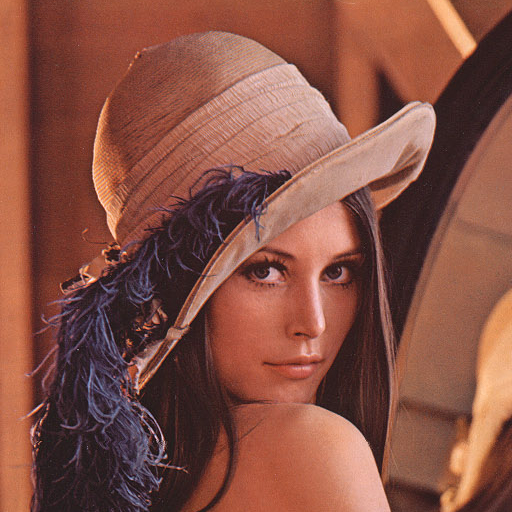
\includegraphics[width=0.4\textwidth]{imagenes/lena32.jpg}\label{fig:f5}}
  \hfill
  \subfloat[LDR]{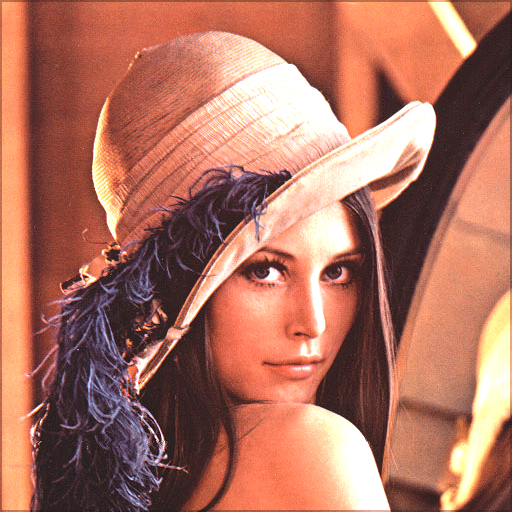
\includegraphics[width=0.4\textwidth]{imagenes/lena32ldr.jpg}\label{fig:f6}}
  \caption{$\alpha$: 255}
\end{figure}


Para reducir errores de redondeo, la division debe será la última operación en realizarse.
El resultado final será saturado de ahi $max$ y $min$ en la primer fórmula.

Además, dado que en los bordes no es posible calcular $ldr$ por la ausencia de vecinos, se devolverá
el valor original. Es decir:

\begin{center}
$O_{i,j}^{K} = I_{i,j}^{K}$ si $i<2 \vee j<2 \vee i+2 \leq tamy \vee j +2 \leq tmax$
\end{center}

(con i indexado a partir de 0)

\subsubsection{Assembler SIMD}

En la implementación de $ldr$ tenemos varios inconvenientes a solventar, pero el principal es el cálculo de la suma. Para lograr aprovechar el paralelismo que ofrece SIMD se realizan varias operaciones.
Para cada fila del cuadrado que supone la sumatoria, se obtienen 4 pixeles en un registro $xmm$ y luego se separan en dos registros diferentes, de manera tal que tengamos el los pixeles $p0$ y $p1$ en uno y $p2$ y $p3$ en otro con cada canal transformado a 16 bits. Para realizarlo se realiza un shuffle para cada caso.\\

Una vez obtenidos los dos registros anteriores, se suman horizontalmente los registros respectivos una vez y se transforma el resultado a 32 bits. Luego se aplican sumas verticales valiendose de un registro de respaldo y varios shifts para eliminar las sumas que no signifiquen en la fórmula.\\

Debido a que la suma que buscamos es de cinco pixeles, se obtiene el 5to pixel en otro registro y se lo opera de manera similar a los anteriores para luego sumarlo a los mismos acumulando la suma de cada fila en el registro particular $xmm0$

\begin{codesnippet}
\begin{verbatim}
.cincoHorizontal:

	; 16  12   8   4   0
	; Li4|Li3|Li2|Li1|Li0
    ;VERSION STANDARD: Con 2 accesos - acceso extra para el pixel 5
    movdqu xmm1, [rdi + r12*pixelSize] ; Li3|Li2|Li1|Li0

	movdqu xmm9, xmm1
	pshufb xmm9, xmm6 ; 0|0|0|r1|0|g1|0|b1|0|0|0|r0|0|g0|0|b0
	phaddw xmm9, xmm11 ; 0|0|0|0|0+r1|g1+b1|0+r0|g0+b0
	pshufb xmm1, xmm7 ; 0|0|0|r3|0|g3|0|b3|0|0|0|r2|0|g2|0|b2
    phaddw xmm1, xmm11 ; 0|0|0|0|r3|g3+b3|r2|g2+b2
    punpcklwd xmm9, xmm11 ; r1|g1+b1|r0|g0+b0
    punpcklwd xmm1, xmm11 ; r3|g3+b3|r2|g2+b2
    paddd xmm1, xmm9 ; r3+r1|g3+b3+g1+b1|r2+r0|g2+b2+g0+b0
    movdqu xmm9, xmm1
    psrldq xmm9, 8 ; 0|0|r3+r1|g3+b3+g1+b1
    paddd xmm1, xmm9 ; r3+r1|g3+b3+g1+b1|r2+r0+r3+r1|g2+b2+g0+b0+g3+b3+g1+b1
    pslldq xmm1, 8 ; r2+r0+r3+r1|g2+b2+g0+b0+g3+b3+g1+b1|0|0
    psrldq xmm1, 8 ; 0|0|r2+r0+r3+r1|g2+b2+g0+b0+g3+b3+g1+b1
	movd xmm9, [rdi + r12*pixelSize + 16] ; 0|0|0|0|0|0|0|0|0|0|0|0|a4|r4|g4|b4

	pslldq xmm9, 12 ; a4|r4|g4|b4|0|0|0|0|0|0|0|0|0|0|0|0
	pand xmm9, xmm8 ; 0|r4|g4|b4|0|0|0|0|0|0|0|0|0|0|0|0
	pshufb xmm9, xmm7 ; 0|0|0|r4|0|g4|0|b4|0|0|0|0|0|0|0|0
	phaddw xmm9, xmm11 ; 0|0|0|0|r4|g4+b4|0|0
	punpcklwd xmm9, xmm11 ; 0|r4|0|g4+b4|0|0|0|0
	psrldq xmm9, 8 ; 0|0|r4|g4+b4
	paddd xmm1, xmm9 ; 0|0|r2+r0+r3+r1+r4|g2+b2+g0+b0+g3+b3+g1+b1+g4+b4
	movdqu xmm9, xmm1
	psrldq xmm9, 4 ; 0|0|0|r2+r0+r3+r1+r4
	paddd xmm1, xmm9 ; 0|0|r2+r0+r3+r1+r4|g2+b2+g0+b0+g3+b3+g1+b1+g4+b4+r2+r0+r3+r1+r4
	pslldq xmm1, 12 ; g2+b2+g0+b0+g3+b3+g1+b1+g4+b4+r2+r0+r3+r1+r4|0|0|0
	psrldq xmm1, 12 ; 0|0|0|g2+b2+g0+b0+g3+b3+g1+b1+g4+b4+r2+r0+r3+r1+r4
	paddd xmm0, xmm1 ; suma hasta la i-esima fila para el pixel ij.

	add r12, r15
	inc r10
	cmp r10, 5
	jl .cincoHorizontal
    
\end{verbatim}
\end{codesnippet}

Una vez obtenida la suma, que al final tendrá un tamaño de 32 bits, se procede a realizar la fórmula de $ldr$. 
El primer paso es armar la un registro con el valor de $alfa$ en sus primeras tres posiciones menos significativas que es donde se encontraran los valores de los canales. Asi mismo, se crea un registro con el divisor $max$ en las cuatro posiciones debido a que con el realizaremos la division.\\

Se crea un registro con la suma replicada en las tres posiciones menos significativas y se procede a calcular la fórmula, para lo cual tenemos la siguiente consideración:\\
 
Debido a que, $canal x sumargb x alfa$ cabe perfectamente dentro de un entero de 32 bits (el máximo es 75x255x255x255 o 75x255x255x-255 = +-1,243,603,125 $\in$ $[$-2,147,483,648 a 2,147,483,647$]$, no se convierte a punto flotante si no hasta la division, por lo tanto será la única operacion de punto flotante del algoritmo, aunque vale mencionar que si por cada pixel, exceptuando las primeras y últimas dos filas y columnas se aplica esta fórmula en total habrá 3x(filas-2)x(columnas-2) operaciones de punto flotante. Para una imagen de 512$x$512 supone 780300 divisiones de punto flotante, que se asemeja bastante a la cantidad de operaciones de punto flotante de $sepia$.


\begin{codesnippet}
\begin{verbatim}

punpcklbwAndCleanAlpha: DB 0x00, 0x88, 0x01, 0x89, 0x02, 0x8A, 0x83, 0x8B, 0x04, 0x8C, 0x05, 0x8D, 0x06, 0x8E, 0x87, 0x8F 
punpckhbwAndCleanAlpha: DB 0x08, 0x81, 0x09, 0x82, 0x0A, 0x83, 0x8B, 0x84, 0x0C, 0x85, 0x0D, 0x86, 0x0E, 0x87, 0x8F, 0x88 
saveOnePixelShifter: DB 0x00, 0x00, 0x00, 0x00, 0x00, 0x00, 0x00, 0x00, 0x00, 0x00, 0x00, 0x00, 0xFF, 0xFF, 0xFF, 0x00
repeatDw: DB 0x00, 0x01, 0x02, 0x03, 0x00, 0x01, 0x02, 0x03, 0x00, 0x01, 0x02, 0x03, 0x00, 0x01, 0x02, 0x03
maxValue: DD 0x004A6A4B ; check this 4876875

section .text
;void _ldr_asm    (
	;unsigned char *src, rdi
	;unsigned char *dst, rsi
	;int cols, edx
	;int filas, ecx
	;int src_row_size, r8d -> no se usa
	;int dst_row_size, r9d -> no se usa
	;int alpha) rsp-8

	; r8 posicion actual
	; r9 contador columnas

_ldr_asm:
	push rbp
	mov rbp, rsp
	push rbx
	push r12
	push r13
	push r14
	push r15

	xor rbx, rbx
	xor r12, r12
	xor r13, r13
	xor r14, r14
	xor r15, r15
	
	mov ebx, [rbp+16] ; alpha
	mov r13d, [maxValue] ; MAX

	cmp ebx, -255
	jl .sinCambios
	cmp ebx, 255
	jg .sinCambios
	cmp edx, 4
	jle .sinCambios ; si tengo menos de cuatro filas terminar.
	cmp ecx, 4
	jle .sinCambios ; si tengo menos que cuatro columnas terminar.

	xor r8, r8 ; posicion actual
	xor r9, r9 ; j = 0
	mov r8d, edx ; r8 = cols

	mov r15d, edx ; r15d = cols
	xor rdx, rdx
	mov r14d, ecx ; r14d = filas.
	sub r14d, 2 ; filas-2
	xor rax, rax ; limpio para usar en multiplicacion.
\end{verbatim}
\end{codesnippet}

\begin{codesnippet}
\begin{verbatim}
	mov eax, r15d
	mul r14d ; edx:eax = r15d*r14d = cols*(filas-2).
	mov ecx, edx
	shl rdx, 32
	mov ecx, eax ; ecx = r15d*r14d = cols*(filas-2). contador loop.

	xor r11, r11
	mov r11d, r15d
	sub r11d, 2 ; cols-2 = colsToProccess

	shl r8, 1 ; r8*2 = i = 2 - j = 0

	movdqu xmm6, [punpcklbwAndCleanAlpha]
	movdqu xmm7, [punpckhbwAndCleanAlpha]
	movdqu xmm8, [saveOnePixelShifter]
	movdqu xmm2, [repeatDw]
	movdqu xmm15, xmm8 ; 0|FF|FF|FF|0|0|0|0|0|0|0|0|0|0|0|0
    psrldq xmm15, 12 ; 0|0|0|0|0|0|0|0|0|0|0|0|0|FF|FF|FF
    movdqu xmm4, xmm8
    psrldq xmm4, 14
    pslldq xmm4, 3 ; 0|0|0|0|0|0|0|0|0|0|0|0|FF|0|0|0

	pxor xmm11, xmm11
	pxor xmm12, xmm12
	pxor xmm13, xmm13

.ciclo: ; while(r8 < rcx) == (actual < total) 
; if(j > 1)
	cmp r9, 2
	jl .menorAColDos
	; estoy en rango.
	mov r12, r8 ; posicion actual
	sub r12, r15
	sub r12, r15 ; posicion actual - dos filas
	sub r12, 2 ; me corro -2 posiciones
	xor r10, r10 ; cuento hasta 5

	pxor xmm0, xmm0
  
    
   ; SUMA CINCO HORIZONTAL    
    
	movd xmm12, ebx
	pshufb xmm12, xmm2 ; alpha|alpha|alpha|alpha

	movd xmm13, r13d
	pshufb xmm13, xmm2 ; max|max|max|max

	movdqu xmm5, xmm0
	pshufb xmm5, xmm2 ; sumargb|sumargb|sumargb|sumargb 

	pxor xmm14, xmm14
	movd xmm14, [rdi + r8*pixelSize] ; 0|0|0|0|0|0|0|0|0|0|0|0|a|r|g|b <- get pixel ij

	movdqu xmm0, xmm14 ; 0|0|0|0|0|0|0|0|0|0|0|0|a|r|g|b
	pand xmm0, xmm15 ; 0|0|0|0|0|0|0|0|0|0|0|0|0|r|g|b
\end{verbatim}
\end{codesnippet}

\begin{codesnippet}
\begin{verbatim}
	punpcklbw xmm0, xmm11 ; 0|0|0|0|0|r|g|b
	punpcklwd xmm0, xmm11 ; 0|r|g|b

	pmulld xmm5, xmm0 ; 0|sumargb*r|sumargb*g|sumargb*b == 0|sumargb*r|sumargb*g|sumargb*b -- maximo posible por dword 75*255*255 = 4876875 in  [-2,147,483,648 to 2,147,483,647]
	pmulld xmm5, xmm12 ; 0|alpha*sumargb*r|alpha*sumargb*g|alpha*sumargb*b <- puede cambiar el signo segun alpha. -- maximo posible por dword 75*255*255*255 or 75*255*255*-255 = +-1,243,603,125 in  [-2,147,483,648 to 2,147,483,647]

    cvtdq2ps xmm5, xmm5 ; 0|fp(alpha*sumargb*r)|fp(alpha*sumargb*g)|fp(alpha*sumargb*b)
	cvtdq2ps xmm13, xmm13 ; fp(max)|fp(max)|fp(max)|fp(max)

	divps xmm5, xmm13 ; 0|(alpha*sumargb*r)/max|(alpha*sumargb*g)/max|(alpha*sumargb*b)/max

	cvtdq2ps xmm0, xmm0 ; 0|fp(r)|fp(g)|fp(b)

	addps xmm5, xmm0 ; 0|r+(alpha*sumargb*r)/max|g+(alpha*sumargb*g)/max|b+(alpha*sumargb*b)/max

	cvttps2dq xmm5, xmm5 ; cast to dw signed 

	packusdw xmm5, xmm11 ; 0|0|0|0|0|r+(alpha*sumargb*r)/max|g+(alpha*sumargb*g)/max|b+(alpha*sumargb*b)/max
	packuswb xmm5, xmm11 ; 0|0|0|0|0|0|0|0|0|0|0|0|0|r+(alpha*sumargb*r)/max|g+(alpha*sumargb*g)/max|b+(alpha*sumargb*b)/max <- tengo los canales calculados saturados a byte.

	pand xmm14, xmm4 ; 0|0|0|0|0|0|0|0|0|0|0|0|a|0|0|0
	por xmm14, xmm5 ; 0|0|0|0|0|0|0|0|0|0|0|0|a|r+(alpha*sumargb*r)/max|g+(alpha*sumargb*g)/max|b+(alpha*sumargb*b)/max

    movd [rsi + r8*pixelSize], xmm14

	inc r9
	inc r8
	cmp r9, r11
	je .igualAColsToProccess ; mayor igual a colsToProccess
	jmp .seguir
    
\end{verbatim}

\end{codesnippet}

\subsubsection{C}

Como ya hemos explicado, C compilado en modo default, carece de paralelismo en las operaciones y por lo tanto $ldr$ se resolverá obteniendo cada pixel y operando unitariamente. Al final el agoritmo es similar pero con más accesos a memoria para lectura y escritura y operaciones de punto flotante unitarias.

\begin{codesnippet}
\begin{verbatim}
                
                int i = 0;
                int indexSquare = c - ((cols*2)+2);
                int sumargb = 0;
                
                while (i < 5) {
                    sumargb += src[indexSquare*4];
                    sumargb += src[indexSquare*4+1];
                    sumargb += src[indexSquare*4+2];
                    sumargb += src[indexSquare*4+4];
                    sumargb += src[indexSquare*4+5];
                    sumargb += src[indexSquare*4+6];
                    sumargb += src[indexSquare*4+8];
                    sumargb += src[indexSquare*4+9];
                    sumargb += src[indexSquare*4+10];
                    sumargb += src[indexSquare*4+12];
                    sumargb += src[indexSquare*4+13];
                    sumargb += src[indexSquare*4+14];
                    sumargb += src[indexSquare*4+16];
                    sumargb += src[indexSquare*4+17];
                    sumargb += src[indexSquare*4+18];
                    indexSquare += cols; //siguiente fila.
                    i++;
                }

                float sumargbf = sumargb;
                float alphaf = alpha;
                float maxf = 4876875;
                float b = (float)src[c*4];
                float g = (float)src[c*4+1];
                float r = (float)src[c*4+2];
                unsigned char a = src[c*4+3];

                b = b + (alphaf*sumargbf*b)/maxf;

                b = MIN(MAX(b,0), 255);

                g = g + (alphaf*sumargbf*g)/maxf;

                g = MIN(MAX(g,0), 255);

                r = r + (alphaf*sumargbf*r)/maxf;

                r = MIN(MAX(r,0), 255);

                dst[c*4] = (unsigned char)b;
                dst[c*4+1] = (unsigned char)g;
                dst[c*4+2] = (unsigned char)r;
                dst[c*4+3] = a;
                
\end{verbatim}
\end{codesnippet}

\subsection{Análisis experimental}

En general, al aplicar filtros sobre imagenes, la performance puede verse afectada por varios motivos, como por ejemplo el scheduler del sistema, que puede generar caidas en el tiempo debido a que debe realizar operaciones de mayor prioridad antes de poder retornar al algoritmo. Cuestiones como esta, serán tenidas en cuenta en la toma de mediciones.\\

Como bien se sabe, la mayoria de los procesadores poseen una memoria integrada que es la más rápida luego de los registros, conocida como memoria caché, y que se subdivide en dos niveles: L1 (a su vez subdividida en datos e instrucciones) y L2 para datos. 
La idea de la misma es tener $"$a mano$"$ datos que sean pedidos al sistema, trayendo consigo además los contiguos en un bloque de memoria (principio de vecinidad espacial), de manera tal que al consultar por el mismo nuevamente o algún contiguo, se obtenga mucho más rápido desde esta memoria. Pero cuando los mismos no se encuentran, el procesador tiene que buscarlos en la memoria ram, siendo este proceso la causa en la caida de performance que más suele afectar a los algoritmos.\\ 

Este último y algunas cuesitones  más serán de estudio en este informe. Para ello introduciremos cada una de las hipótesis que se plantearán en base a lo que cada implementación en particular genere y propondremos un test a realizar, explicando la metodologia para llevarlo a cabo y los resultados obtenidos con las conclusiones que correspondan.\\
 
Además, escogeremos una implementación en particular para llevar a cabo algunos tests especiales que surjan en base a resultados más o menos generales para tener una vision extra de lo que sucede en esos casos.\\

\subsubsection{Metodologias}

Evaluaremos con los distintos tests el rendimiento de cada implementación. El mejor o peor rendimiento de las implementaciones se basa en la toma de tiempos de ejecución. Como los tiempos de ejecución son relativamente pequeños, en general, se utilizará uno de los contadores de performance que posee el procesador. \\

Cada vez que se corra un filtro se tomará la diferencia entre el comienzo y el final del proceso y se dividirá este valor por la cantidad de pixeles de la imagen (resolución de la imagen) para poder analizar todas las muestras en la misma unidad ($tics de reloj /cantidad de pixeles$) y que además nos permitirá observar mejor cambios en el comportamiento de las muestras.\\

Luego al conjunto de mediciones tomadas para una misma imagen calcularemos una media $\alpha$-podada 0.5 (promedio intercuartil) sobre el total de las corridas de un experimento. La poda se realizará a derecha, eliminando así los outliers más grandes que puedan existir (las muestras se ordenan de menor a mayor). Lo cual es más que suficiente para 100 iteraciones sobre una imagen (que es la cantidad de iteraciones que utilizaremos en todos los tests), que nos deja 50 muestras luego de aplicar la poda. \\ 
Además tomaremos el desvio standard muestral, utilizando el mismo set de datos al que aplicamos la poda $\alpha$, para poder medir que dispersion tienen los mismos con respecto a la media. 
De esta manera podremos saber que si la dispersion de los datos es muy grande, para dos curvas aparentemente distanciadas en promedio, tal vez no haya diferencias sigificativas.

La imagen elegida para los tests será la siguiente:.

\newpage

\begin{figure}
  \begin{center}
	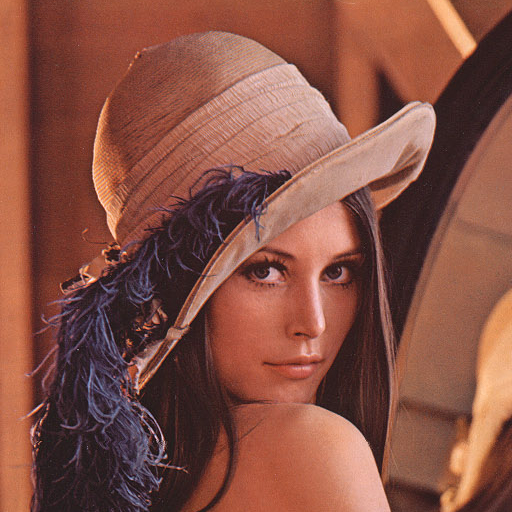
\includegraphics[scale=.5]{imagenes/lena32.jpg}
	\caption{Lena}
	\label{lena}
  \end{center}
\end{figure}

El procesador utilizado para realizar todos los tests sera un Intel(R) Core(TM) Intel Core i5-2430M @ 2.40GHz con caché L2 de 3MB.

Para que la caché no influya en cada corrida se implementó un algoritmo sencillo que lo que hará es ocupar la caché L2 antes de cada corrida. Sabiendo que la caché es de 3MB el algoritmo siguiente debería garantizar que la caché se ocupará con información que no altere los resultados de los tests. \\
Además cambiando el valor de la variable $fria$ por uno podremos testear la cache precalentada con la imagen de testeo para ver como influye en los tiempos de proceso de cada algoritmo el estar la imagen cacheada totalmente o parcialmente.

\begin{codesnippet}
\begin{verbatim}
                
  				int fria = 1;
				if (fria == 1) {
					char *basura = (char*)malloc(sizeof(char)*786432);
					srand(5);
					int i = 0;
					while (i < 786432) {
						basura[i] = rand() % 27;            
						i++;                
					}
					long int suma = 0;
					i = 0;                
					while (i < 786432) {
						suma += basura[i];   
						i++;         
					}
					free(basura);
				}else {
					unsigned int *src_matrix = config->archivo_entrada;
					unsigned int size = sizeof(config->archivo_entrada);
					int argbSum = 0;
					for (int i = 0; i < size; i++)
					{
						int argb = src_matrix[i];
						argbSum += argb;
					}
				}
                
\end{verbatim}
\end{codesnippet}

\pagebreak

\subsubsection{Cosideraciones}

Para que las comparaciones entre código $asm$ y $C$ sean más justas, utilizaremos como version default de código $C$ flag de optimización $O1$. El motivo de esta elección es que el código generado por $O0$ no realiza grandes optimizaciones y solo utiliza $SIMD$ para escalares por lo cual la performance es muy baja. \\

De todas maneras, uno de los fines de este informe es mostrar que sin flags de optimización, sería a día de hoy casi imposible realizar, por ejemplo, reproducción de video en tiempo real con gran carga de procesamiento en un computador de sobremesa. Es decir, que código generado con $SIMD$ ya sea por un programador o por el compilador con ayuda de flags de optimización es muy importante para esta problematica.\\

Veamos entonces cuanta diferencia existe entre flags $O1$ y $O0$ para cada filtro.

\begin{figure}[h]
  \begin{center}
	\includegraphics[scale=0.5]{ldrClocksO1VsO0.pdf}
  \end{center}
\end{figure}

\begin{figure}[h]
  \begin{center}
	\includegraphics[scale=0.5]{sepiaClocksO1VsO0.pdf}
  \end{center}
\end{figure}
 
\begin{figure}[h]
  \begin{center}
	\includegraphics[scale=0.5]{cropflipClocksO1VsO0.pdf}
  \end{center}
\end{figure}
 
Como podemos notar, se logran eficiencias elevadas utilizando solamente $O1$ y en principio podriamos lograr más eficiencia utilizando $O2$ y $O3$. Así que por fines prácticos eligiremos el último para ver que tan lejos podemos llegar.\\ 
 
\subsection{Hipótesis}


\subsubsection{Comportamiento: Aumentando resoluciones}

Nos interesa saber como se comportan los algoritmos para cada filtro en sus dos variantes ($asm$, $C-O1$) cuando se varia el tamaño de ~\ref{lena}. Es decir, analizaremos el comportamiento de los algoritmos frente a variaciones de tamaño\\

El resultado esperado para todos los filtros en ambas versiones es que el tiempo aumente linealmente para aumentos lineales en el tamaño de las imágenes. En particular como lo que haremos será tomar cada medición como $tics /(ancho \times alto)$ esta linealidad será en realidad una constante sobre las mediciones. 

Es decir que no varia el tiempo para un pixel si no que varia el tiempo en funcion de la cantidad total de pixeles.

Además, sería deseable que la version implementada en $asm$ se mantenga por encima en performance (por debajo en cuanto a tiempos) de $C-O1$. \\ 
En cropflip, en particular, tomaremos un tamaño proporcional a la imagen de corte para realizar las mediciones que será proporcional al tamaño de la imagne original: \\

\begin{enumerate}
\item $width-16$ 
\item $height-16$
\item $offsetY: 16$
\item $offsetX: 16$
\end{enumerate}

De manera que el corte varie con el tamaño. 

\subsubsection{Performance caché: caliente vs. fria}

El fin de este test es ver si existen diferencias entre correr los algoritmos con la cache en frio (es decir sin la imagen previamente leida) con respecto a caché caliente (imagen previamente leida). \\

A priori, el principio de localidad espacial con el cual trabaja la memoria caché podría hacer que la diferencia entre ambos tests no sea tan notable. 
Sabemos que una linea de caché en un procesador intel es de 64 bytes, por lo cual podremos almacenar hasta 16 pixeles en una linea. Veremos luego de los tests con más detalle porque podría influir esto.

Para $cropflip$ tomaremos el corte de la misma manera que se realizará en el test de resoluciones.
La version de código utilizada en estos tests será en $asm$.

\subsubsection{Performance: implementaciones y filtros}

Como se comentó, el principal objetivo del informe es comprobar si $assembler$ $SIMD$ supone una ventaja frente a código compilado sin flags de optimización. 
Hemos podido comprobar que con flags $O1$ se obtiene una performance elevada frente a $O0$.\\

En este test correremos todos los filtros comparando sus versiones de $assembler$ $SIMD$ contra $C-O1$ y además incluiremos $C$ con flags de optimización $O3$ para ver que tan bien puede optimizar el compilador. \\
La idea es ver que ventaja supone programar a mano en $SIMD$ frente a utilizar flags de optimización en el proceso de compilación.\\ 

\subsubsection{Performance: versiones de $ldr$}

Elegimos el filtro $sepia$ para analizar dos teorias relacionadas a SIMD. 

$A)$ Deseamos ver que sucede si igualamos la cantidad de accesos a memoria de la imagen en la implementacion de $assembler$ $SIMD$ a la de $C-O1$ (es decir, cambiando los accesos de a 128 bits por accesos de 32 bits) manteniendo las operaciones de los pixeles sin cambios  y ver si aún asi la version de $assembler$ $SIMD$ sigue siendo más óptima.

El mótivo de este test es comprobar que el principio de localidad espacial se cumple, es decir, que al acceder a una posición de memoria, una linea completa se cargará en memoria caché, por lo cual no importa si accedemos con instrucciones de 128 o 32 bits, siempre estaremos accediendo a la caché para las posiciones de memoria contiguas.

El código $assembler$ $SIMD$ sin accesos empaquetados cambia de la siguiente manera:

\begin{codesnippet}
\begin{verbatim}

		;mascaras
		movd xmm7, [alfainv]
 	    pslldq xmm7, 4
	    movd xmm7, [alfainv + 4]
	    pslldq xmm7, 4
	    movd xmm7, [alfainv + 8]
	    pslldq xmm7, 4
	    movd xmm7, [alfainv + 12]
	    pslldq xmm7, 4

	    movd xmm8, [alfamasc]
	    pslldq xmm8, 4
	    movd xmm8, [alfamasc + 4]
	    pslldq xmm8, 4
	    movd xmm8, [alfamasc + 8]
	    pslldq xmm8, 4
	    movd xmm8, [alfamasc + 12]
	    pslldq xmm8, 4

	    movd xmm0, [factores]
	    pslldq xmm0, 4
	    movd xmm0, [factores + 4]
	    pslldq xmm0, 4
	    movd xmm0, [factores + 8]
	    pslldq xmm0, 4
	    movd xmm0, [factores + 12]
	    pslldq xmm0, 4

		;leer de memoria pixeles
		;movdqu xmm1, [rdi]; XMM1 = | p3 | p2 | p1 | p0 |
		movd xmm1, [rdi]
		pslldq xmm1, 4
		movd xmm1, [rdi + 4]
		pslldq xmm1, 4
		movd xmm1, [rdi + 8]
		pslldq xmm1, 4
		movd xmm1, [rdi + 12]	
		
		;;;;;;;;;;;;;;;;;;;;;;;;;;;;;;;;;;;;;
		
		;escribir a memoria pixeles
		;movdqu [rsi], xmm1
		movd [rsi], xmm1
		psrldq xmm1, 4
		movd [rsi + 4], xmm1
		psrldq xmm1, 4
		movd [rsi + 8], xmm1
		psrldq xmm1, 4
		movd [rsi + 12], xmm1

\end{verbatim}
\end{codesnippet}

Veamos que el código $C$ compilado con $O1$ tiene una cantidad de accesos para lectura y escritura a memoria similar a la de $assember$ $SIMD$ modificado

\begin{codesnippet}
\begin{verbatim}

<sepia_c>:
test   ecx,ecx
jle    114 <sepia_c+0x114>
push   r15
push   r14
push   r13
push   r12
push   rbp
push   rbx
movsxd r13,r8d
movsxd r14,r9d
mov    rbp,rsi
mov    rbx,rdi
mov    r12d,0x0
movsd  xmm7,QWORD PTR [rip+0x0]        # 2c <sepia_c+0x2c>

movsd  xmm6,QWORD PTR [rip+0x0]        # 34 <sepia_c+0x34>

movsd  xmm5,QWORD PTR [rip+0x0]        # 3c <sepia_c+0x3c>

movapd xmm4,xmm6
movsd  xmm3,QWORD PTR [rip+0x0]        # 48 <sepia_c+0x48>

movapd xmm2,xmm6
mov    r9d,0xffffffff
jmp    f5 <sepia_c+0xf5>
mov    BYTE PTR [r11],al
movzx  eax,BYTE PTR [r10+0x3]
mov    BYTE PTR [r11+0x3],al
add    r8d,0x1
cmp    edx,r8d
je     e6 <sepia_c+0xe6>
lea    r10d,[r8*4+0x0]

movsxd r10,r10d
lea    r11,[rdi+r10*1]
add    r10,rsi
movzx  eax,BYTE PTR [r10+0x2]
movzx  r15d,BYTE PTR [r10+0x1]
add    eax,r15d
movzx  r15d,BYTE PTR [r10]
add    eax,r15d
pxor   xmm0,xmm0
cvtsi2sd xmm0,eax
movapd xmm1,xmm0
mulsd  xmm1,xmm7
mov    eax,r9d
ucomisd xmm1,xmm6
ja     af <sepia_c+0xaf>
cvttsd2si eax,xmm1
mov    BYTE PTR [r11+0x2],al
movapd xmm1,xmm0
mulsd  xmm1,xmm5
mov    eax,r9d
ucomisd xmm1,xmm4
ja     c8 <sepia_c+0xc8>  
\end{verbatim}
\end{codesnippet}


\begin{codesnippet}
\begin{verbatim}


cvttsd2si eax,xmm1
mov    BYTE PTR [r11+0x1],al
mulsd  xmm0,xmm3
mov    eax,r9d
ucomisd xmm0,xmm2
ja     57 <sepia_c+0x57>
cvttsd2si eax,xmm0
jmp    57 <sepia_c+0x57>
add    r12d,0x1
add    rbp,r14
add    rbx,r13
cmp    ecx,r12d
je     10a <sepia_c+0x10a>
test   edx,edx
jle    e6 <sepia_c+0xe6>
mov    rdi,rbp
mov    rsi,rbx
mov    r8d,0x0
jmp    6c <sepia_c+0x6c>
pop    rbx
pop    rbp
pop    r12
pop    r13
pop    r14
pop    r15
repz ret 

\end{verbatim}
\end{codesnippet}

$B)$ Deseamos ver que sucede si en lugar de dividir en punto flotante empaquetados se reemplaza esa seccion de código por operaciones con enteros empaquetados: que version tiene mejor rendimiento? $assembler$ con ops de punto flotante o $assembler$ con ops en enteros?

Para llevarlo a cabo cambiaremos los valores del filtro que se aplican a cada canal: 0.2, 0.3, 0.5 por 2, 2, 2 en ambas versiones, dado que, para la version de enteros no disponemos de punto flotante y queremos tener una representación de la cual conozcamos los valores que manejamos.\\
Lo que si no haremos en la version de punto flotante será convertir los valores de los canales a enteros luego de aplicar la operación y no empaquetaremos en ninguna de las dos versiones los resultados que se obtengan. De esta manera eliminaremos la mayor cantidad de proceso extra para que las comparaciones sean lo más justas posibles.  
Luego todo será igual, pero a la ahora de aplicar el filtro la version de enteros será:\\

\begin{codesnippet}
\begin{verbatim}
                
		pmulld xmm1, xmm0; XMM1 = |*|suma0*2|suma0*2|suma0*2|  
		pmulld xmm2, xmm0; XMM2 = |*|suma2*2|suma2*2|suma2*2|  
		pmulld xmm3, xmm0; XMM3 = |*|suma1*2|suma1*2|suma1*2|   
		pmulld xmm4, xmm0; XMM4 = |*|suma3*2|suma3*2|suma3*2|   
                
\end{verbatim}
\end{codesnippet}

Y la version de punto flotante será:

\begin{codesnippet}
\begin{verbatim}

		mulps xmm1, xmm0; XMM1 = |*|suma0*2|suma0*2|suma0*2|  
		mulps xmm2, xmm0; XMM2 = |*|suma2*2|suma2*2|suma2*2|  
		mulps xmm3, xmm0; XMM3 = |*|suma1*2|suma1*2|suma1*2|  
		mulps xmm4, xmm0; XMM4 = |*|suma3*2|suma3*2|suma3*2|     

\end{verbatim}
\end{codesnippet}
